\documentclass[tikz,border=2pt]{standalone}

\usepackage{pgfplots}
\pgfplotsset{compat=1.18}

\begin{document}
	
	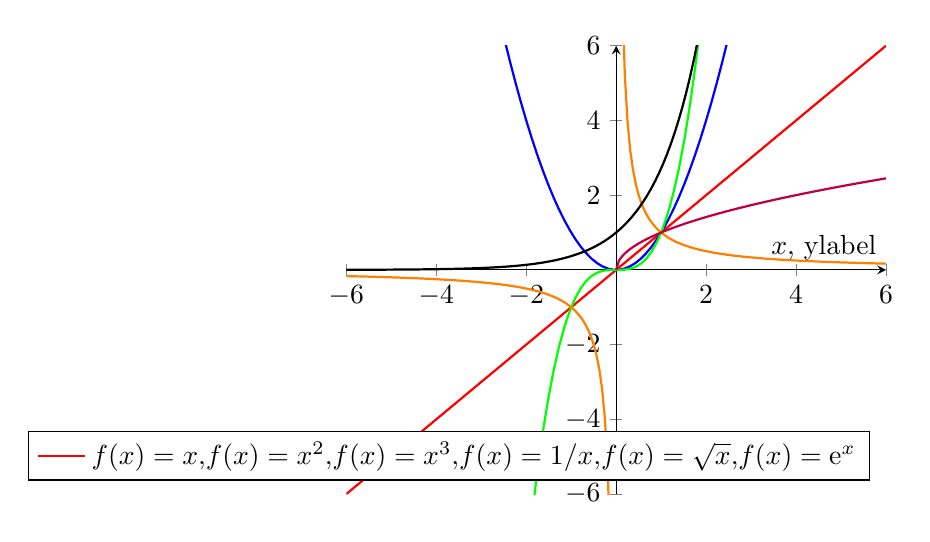
\begin{tikzpicture}
		\begin{axis}[
			xmin=-6,xmax=6,
			ymin=-6,ymax=6,
			axis lines=middle,
			xlabel=$x\text{,}$
			ylabel=$y\text{,}$
			legend style={yshift=-25pt,font=\small},
			legend pos=south east,
			legend cell align={left}
			]
			\addplot[thick,domain=-6:6, samples=100, color=red]{x};
			\addplot[thick,domain=-6:6, samples=100, color=blue]{x*x};
			\addplot[thick,domain=-6:6, samples=100, color=green]{x*x*x};
			\addplot[thick,domain=0.01:6, samples=100, color=orange]{1/x};
			\addplot[thick,domain=0:6, samples=100, color=purple]{sqrt(x)};
			\addplot[thick,domain=-6:2.5, samples=100, color=black]{e^x};
			\legend{$f(x)=x\text{,}$$f(x)=x^2\text{,}$$f(x)=x^3\text{,}$$f(x)=1/x\text{,}$$f(x)=\sqrt{x}\text{,}$$f(x)=\mathrm{e}^x$}
			\addplot[thick,domain=-6:-0.01, samples=100, color=orange]{1/x};
		\end{axis}
	\end{tikzpicture}
	
\end{document}